%!TEX program = xelatex
%!TEX root = ../all_short.tex

\chapter{Some notes on Statistical Learning Theory: A Summary}

\section*{Introduction}
Statistical learning theory provides the theoretical foundation for machine learning, addressing the fundamental question: under what conditions is learning possible? Given a hypothesis class $\mathcal{H}$ and a training set of size $n$, what guarantees can we provide about the quality of the learned predictor? The theory provides precise mathematical answers that apply universally, revealing principles that govern whether and how quickly we can learn.

\section*{Learning Algorithms and the Role of Hypothesis Classes}

\subsection*{Learning Algorithms}
\begin{itemize}
    \item A learning algorithm $\mathcal{A}$ is a procedure that takes training data and produces a predictor.
    \item Algorithms operate within a structured framework called the \alert{hypothesis class} $\mathcal{H}$, which specifies the set of candidate functions the algorithm may choose from.
    \item This constraint is the \alert{inductive bias}: the learner's prior belief about what kind of solution is likely to work.
    \item Notation: $h^{\mathcal{A}}_{\mathcal{T}}$ denotes the predictor returned by algorithm $\mathcal{A}$ when applied to training set $\mathcal{T}$.
\end{itemize}

\subsection*{Empirical Risk Minimization (ERM)}
\begin{itemize}
    \item \textbf{Definition:} ERM returns the predictor in $\mathcal{H}$ that achieves the lowest training error:
    \begin{myequation}
    h_{\mathcal{T}} = \argmin{h \in \mathcal{H}} \overline{\mathcal{R}}_{\mathcal{T}}(h)
    \end{myequation}
    where $\overline{\mathcal{R}}_{\mathcal{T}}(h)$ is the empirical risk (average loss on the training set).
    \item \textbf{Intuition:} Choose the predictor that works well on available data.
    \item \textbf{Danger:} The algorithm may overfit — fitting the training set perfectly while generalizing poorly.
\end{itemize}

\subsection*{The Fundamental Question}
\begin{itemize}
    \item Given $\mathcal{H}$, loss function $L$, and distribution $p$ over the data, can we guarantee that applying a learning algorithm (like ERM) to a sufficiently large training set will produce a predictor with small true risk?
    \item Learnability depends on:
    \begin{enumerate}
        \item The size/complexity of the hypothesis class.
        \item The amount of training data available.
        \item The required accuracy and confidence (error tolerance $\varepsilon$ and confidence parameter $\delta$).
    \end{enumerate}
\end{itemize}

\begin{figure}[ht]
\begin{center}
    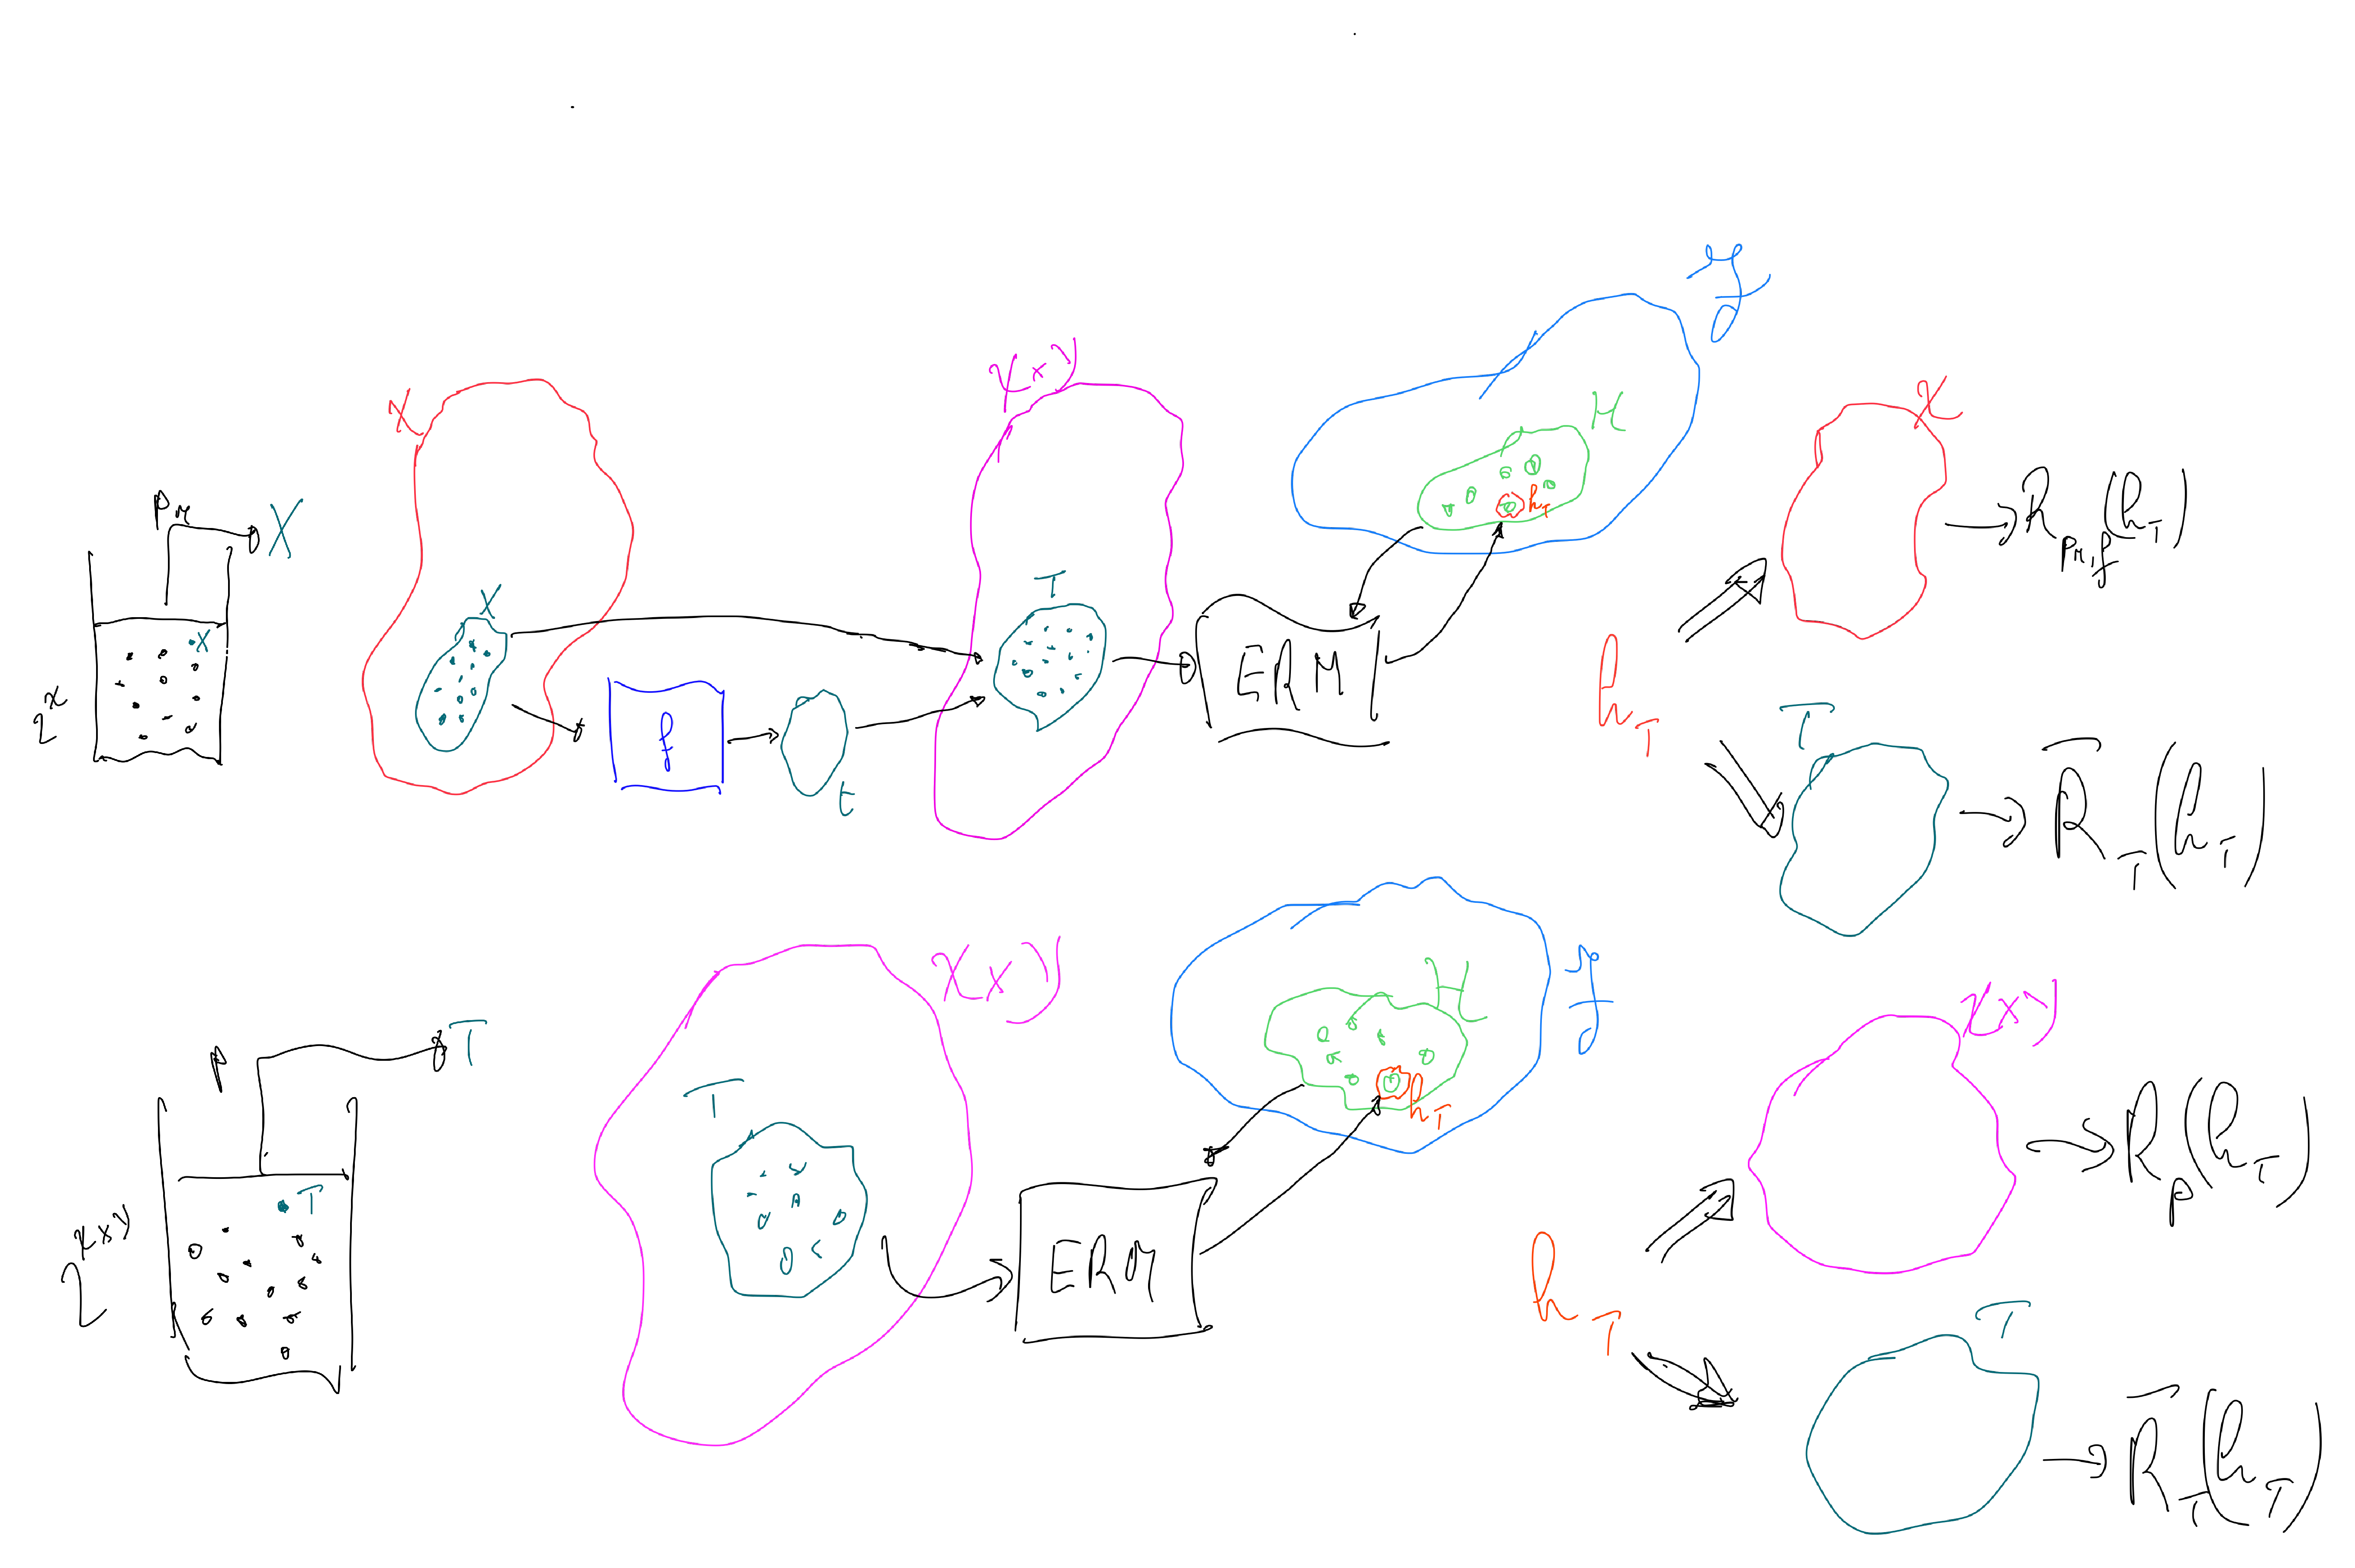
\includegraphics[width=.9\textwidth]{figs/fig1.pdf}
    \caption{Sketch of the learning situation under deterministic (top) and probabilistic (bottom) assumptions.}\label{f:slt}
\end{center}
\end{figure}

\subsection*{Learning with Finite Hypothesis Classes Under Realizability}

\subsubsection*{Realizability Assumption}
\begin{itemize}
    \item There exists some predictor $h^*\in\mathcal{H}$ that makes no error in classifying items in $\mathcal{X}$:
    \begin{myequation}
        \mathcal{R}_{p_{\scalebox{0.4}{$M$}},f}(h^*)=\ev{p_{\scalebox{0.4}{$M$}},f}{L(h^*(\x),f(\x))}=0
    \end{myequation}
    \item For any training set $\mathcal{T}=(\X,\t)$ with $t_i=f(\x_i)$, we have $\overline{\mathcal{R}}_{\mathcal{T}}(h^*)=0$.
    \item This is a strong assumption — it assumes our hypothesis class contains a perfect model of the world.
\end{itemize}

\subsubsection*{ERM Under Realizability}
\begin{itemize}
    \item ERM returns a predictor $h_{\mathcal{T}}$ with zero training error: $\overline{\mathcal{R}}_{\mathcal{T}}(h_{\mathcal{T}})=0$.
    \item However, $h_{\mathcal{T}}$ may not equal $h^*$, and may make errors on elements not in $\mathcal{T}$ ($\mathcal{R}_{p_{\scalebox{0.4}{$M$}},f}(h_{\mathcal{T}})>0$).
    \item ERM might return any predictor from the set of all functions that achieve zero training error — some are genuinely good, others are misleading.
\end{itemize}

\subsubsection*{Bad Predictors and Bad Datasets}
\begin{itemize}
    \item Let $\varepsilon > 0$ be the acceptable error tolerance.
    \item A predictor $h \in \mathcal{H}$ is \alert{bad} if its true risk exceeds $\varepsilon$:
    \begin{myequation}
    \mathcal{R}_{p_M, f}(h) > \varepsilon
    \end{myequation}
    \item Let $\mathcal{H}_B$ denote the set of all bad predictors.
    \item A training set $\mathcal{T}$ is \alert{bad} (misleading) if at least one bad predictor achieves zero training error on it:
    \begin{myequation}
    \exists h \in \mathcal{H}_B: \overline{\mathcal{R}}_{\mathcal{T}}(h) = 0
    \end{myequation}
    \item A training set is \alert{very bad} if applying ERM on it returns a bad predictor.
\end{itemize}

\subsubsection*{Bounding the Probability of a Bad Training Set}
\begin{itemize}
    \item For a single bad predictor $h\in \mathcal{H}_B$, it misclassifies at least a fraction $\varepsilon$ of the population, so it correctly classifies at most a fraction $1-\varepsilon$.
    \item Probability that $h$ correctly classifies all $n$ independent objects: $p_{h}^{n}\leq (1-\varepsilon)^n \le e^{-\varepsilon n}$.
    \item Using the union bound over all bad predictors:
    \begin{myequation}
    \prob{\mathcal{T}\sim p^n}{\exists h \in \mathcal{H}_B: \overline{\mathcal{R}}_{\mathcal{T}}(h) = 0} \le |\mathcal{H}_B| \, e^{-\varepsilon n} \le |\mathcal{H}| \, e^{-\varepsilon n}
    \end{myequation}
    \item Setting $|\mathcal{H}| \, e^{-\varepsilon n} \le \delta$ ensures the probability of a bad training set is at most $\delta$.
    \item Solving for $n$:
    \begin{myequation}\label{eq:sample-complexity-finite}
    n \ge \left\lceil \frac{1}{\varepsilon}\ln\frac{|\mathcal{H}|}{\delta}\right\rceil
    \end{myequation}
    This is the \alert{sample complexity} for learning with finite hypothesis classes under realizability.
\end{itemize}

\subsubsection*{Analysis of Sample Complexity Components}
\begin{itemize}
    \item \textbf{Accuracy ($\varepsilon$):} Appears in denominator — inverse relationship. Halving $\varepsilon$ doubles required sample size.
    \item \textbf{Confidence ($\delta$):} Appears inside logarithm. Reducing $\delta$ by factor $c$ increases sample size by $\frac{1}{\varepsilon}\ln c$ (modest increase).
    \item \textbf{Class complexity ($|\mathcal{H}|$):} Appears as $\ln|\mathcal{H}|$, giving logarithmic relationship. Even large classes remain learnable with reasonable data.
    \item \textbf{Key limitation:} This analysis relies on $\mathcal{H}$ being finite. For infinite classes, we need more sophisticated tools.
\end{itemize}

\subsubsection*{Numerical Examples}
\begin{itemize}
    \item $|\mathcal{H}| = 10,000$, $\varepsilon = 0.1$, $\delta = 0.05$:
    \begin{myequation}
    n \ge \frac{1}{0.1}\ln\frac{10,000}{0.05} = 10 \, \ln(200,000) \approx 122 \text{ examples}
    \end{myequation}
    \item $\varepsilon = 0.02$ (five-fold improvement):
    \begin{myequation}
    n \ge \frac{1}{0.02}\ln(200,000) \approx 50 \times 12.2 = 610 \text{ examples}
    \end{myequation}
    \item $\delta = 0.01$ (99\% confidence) with $\varepsilon = 0.1$:
    \begin{myequation}
    n \ge \frac{1}{0.1}\ln\frac{10,000}{0.01} = 10 \, \ln(1,000,000) \approx 138 \text{ examples}
    \end{myequation}
    (only 16 additional examples for four times higher confidence)
\end{itemize}

\subsection*{PAC Learning: Formalizing Learnability}

\subsubsection*{PAC Learnability Under Realizability}
\begin{definition}[PAC Learnability]
A hypothesis class $\mathcal{H}$ is \alert{PAC learnable} if there exist a function $m_{\mathcal{H}}: (0,1)^2 \to \mathbb{N}$ (the sample complexity function) and a learning algorithm $\mathcal{A}$ such that for every $\varepsilon, \delta \in (0,1)$, every distribution $p_M$ over $\mathcal{X}$, and every labeling function $f: \mathcal{X} \to \{0,1\}$ satisfying realizability (there exists $h^* \in \mathcal{H}$ with $\mathcal{R}_{p_M, f}(h^*) = 0$), when $\mathcal{A}$ is applied to a training set $\mathcal{T}$ of size $n \geq m_{\mathcal{H}}(\varepsilon, \delta)$ generated by sampling $n$ independent examples from $p_M$ and labeling them with $f$, the algorithm returns a predictor $h_{\mathcal{T}}$ such that
\begin{myequation}
\mathcal{R}_{p_M, f}(h_{\mathcal{T}}) \leq \varepsilon
\end{myequation}
with probability at least $1 - \delta$.
\end{definition}

For finite hypothesis classes, ERM is a PAC learning algorithm with sample complexity:
\begin{myequation}
m_{\mathcal{H}}(\varepsilon, \delta) \leq \left\lceil \frac{1}{\varepsilon}\ln\frac{|\mathcal{H}|}{\delta}\right\rceil
\end{myequation}

\subsubsection*{The Bayes Predictor}
\begin{itemize}
    \item In the agnostic (non-realizable) setting, labels are generated stochastically according to conditional probability $p_C(t|\mathbf{x})$.
    \item The \alert{Bayes predictor} minimizes true risk pointwise:
    \begin{myequation}
    h^*(\mathbf{x}) = \argmin{y \in \{0,1\}} \ev{t \sim p_C(\cdot|\mathbf{x})}{L(y, t)}
    \end{myequation}
    \item For binary classification with 0-1 loss:
    \begin{myequation}
    h_{\text{Bayes}}(\mathbf{x}) = \begin{cases} 1 & \text{if } p_C(t=1|\mathbf{x}) \geq 0.5 \\ 0 & \text{otherwise} \end{cases}
    \end{myequation}
    \item The \alert{Bayes risk} $\mathcal{R}^* = \mathcal{R}_p(h_{\text{Bayes}})$ is the irreducible error inherent in the stochasticity of label generation.
    \item The Bayes predictor is unattainable in practice because it requires knowledge of the true conditional distribution.
    \item The \emph{No Free Lunch theorem} shows that without additional assumptions, no algorithm can guarantee finding a predictor as good as Bayes for every distribution.
\end{itemize}

\subsection*{Agnostic PAC Learning}

\subsubsection*{Definition}
\begin{definition}[Agnostic PAC Learnability]
A hypothesis class $\mathcal{H}$ is \alert{agnostic PAC learnable} if there exist a function $m_{\mathcal{H}}: (0,1)^2 \to \mathbb{N}$ and a learning algorithm $\mathcal{A}$ such that for every $\varepsilon, \delta \in (0,1)$ and every distribution $p$ over $\mathcal{X} \times \mathcal{Y}$, when $\mathcal{A}$ is applied to a training set $\mathcal{T}$ of size $n \geq m_{\mathcal{H}}(\varepsilon, \delta)$ generated by sampling $n$ independent pairs from $p$, the algorithm returns a predictor $h_{\mathcal{T}}$ such that
\begin{myequation}
\mathcal{R}_p(h_{\mathcal{T}}) \leq \min_{h \in \mathcal{H}} \mathcal{R}_p(h) + \varepsilon
\end{myequation}
with probability at least $1 - \delta$.
\end{definition}

\begin{itemize}
    \item Compares to the best error achievable within $\mathcal{H}$, denoted $\mathcal{R}_p(h^*) = \min_{h \in \mathcal{H}} \mathcal{R}_p(h)$.
    \item Decomposition: \alert{Approximation error} (how well the best in $\mathcal{H}$ approximates the truth) and \alert{estimation error} (how well we estimate the best in $\mathcal{H}$).
    \item Agnostic PAC learnability generalizes PAC learnability (if realizability holds, $\mathcal{R}_p(h^*) = 0$, reducing to ordinary PAC learning).
\end{itemize}

\subsubsection*{Extension to General Loss Functions}
\begin{definition}[Agnostic PAC Learnability with General Loss]
A hypothesis class $\mathcal{H}$ is \alert{agnostic PAC learnable} with respect to a loss function $L: \mathcal{Y} \times \mathcal{Y} \to [0, M]$ if there exist $m_{\mathcal{H}}: (0,1)^2 \to \mathbb{N}$ and a learning algorithm $\mathcal{A}$ such that for every $\varepsilon, \delta \in (0,1)$ and every distribution $p$ over $\mathcal{X} \times \mathcal{Y}$, when $\mathcal{A}$ is applied to a training set $\mathcal{T}$ of size $n \geq m_{\mathcal{H}}(\varepsilon, \delta)$, it returns $h_{\mathcal{T}}$ satisfying
\begin{myequation}
\mathcal{R}_p(h_{\mathcal{T}}) = \ev{(\mathbf{x}, t) \sim p}{L(h_{\mathcal{T}}(\mathbf{x}), t)}\leq \min_{h \in \mathcal{H}} \ev{(\mathbf{x}, t) \sim p}{L(h(\mathbf{x}), t)}+ \varepsilon
\end{myequation}
with probability at least $1 - \delta$.
\end{definition}

\subsubsection*{Empirical Risk vs True Risk: Representative Training Sets}
\begin{definition}[$\varepsilon$-Representative Sample]
A training set $\mathcal{T}$ is $\varepsilon$-representative with respect to hypothesis class $\mathcal{H}$, loss function $L$, and distribution $p(\mathbf{x}, t)$ if for every predictor $h \in \mathcal{H}$:
\begin{myequation}
\left| \overline{\mathcal{R}}_{\mathcal{T}}(h) - \mathcal{R}_p(h) \right| \leq \varepsilon
\end{myequation}
\end{definition}

\begin{itemize}
    \item Ensures that each predictor's training error differs from its true error by at most $\varepsilon$.
    \item If $\mathcal{T}$ is $\frac{\varepsilon}{2}$-representative, then for $h_{\mathcal{T}}$ returned by ERM:
    \begin{enumerate}
        \item $\overline{\mathcal{R}}_{\mathcal{T}}(h^*) \leq \mathcal{R}_p(h^*) + \frac{\varepsilon}{2}$ where $h^* = \arg\min_{h \in \mathcal{H}} \mathcal{R}_p(h)$.
        \item Since ERM minimizes empirical risk: $\overline{\mathcal{R}}_{\mathcal{T}}(h_{\mathcal{T}}) \leq \overline{\mathcal{R}}_{\mathcal{T}}(h^*) \leq \mathcal{R}_p(h^*) + \frac{\varepsilon}{2}$.
        \item By representativeness again: $\mathcal{R}_p(h_{\mathcal{T}}) \leq \overline{\mathcal{R}}_{\mathcal{T}}(h_{\mathcal{T}}) + \frac{\varepsilon}{2} \leq \mathcal{R}_p(h^*) + \varepsilon$.
    \end{enumerate}
    \item Thus, representativeness directly guarantees the agnostic PAC property.
\end{itemize}

\subsubsection*{Uniform Convergence}
\begin{definition}[Uniform Convergence]
A hypothesis class $\mathcal{H}$ has the \alert{uniform convergence} property with respect to a loss function $L$ if there exists a function $m_{\mathcal{H}}^{\text{UC}}: (0,1)^2 \to \mathbb{N}$ such that for every $\varepsilon, \delta \in (0,1)$ and every distribution $p(\mathbf{x}, t)$, if $\mathcal{T}$ is a dataset of $n \geq m_{\mathcal{H}}^{\text{UC}}(\varepsilon, \delta)$ independent pairs drawn from $p$, then with probability at least $1 - \delta$, the sample $\mathcal{T}$ is $\varepsilon$-representative.
\end{definition}

\begin{itemize}
    \item Requires \emph{all} predictors in $\mathcal{H}$ to simultaneously have their empirical risk concentrate around their true risk.
    \item For finite classes, uniform convergence follows from the union bound:
    \begin{myequation}
    m_{\mathcal{H}}^{\text{UC}}(\varepsilon, \delta) \leq \left\lceil \frac{1}{\varepsilon^2} \ln\frac{2|\mathcal{H}|}{\delta}\right\rceil
    \end{myequation}
    \item This bound grows logarithmically in $|\mathcal{H}|$ and as $1/\varepsilon^2$ in accuracy.
    \item The chain of implications:
    \begin{myequation}
    \text{Uniform Convergence} \implies \text{$\varepsilon$-Representativeness} \implies \text{Agnostic PAC Learnability}
    \end{myequation}
    \item More precisely:
    \begin{myequation}
    m_{\mathcal{H}}(\varepsilon, \delta) \leq m_{\mathcal{H}}^{\text{UC}}\left(\frac{\varepsilon}{2}, \delta\right)
    \end{myequation}
    and ERM is a successful agnostic PAC learning algorithm for $\mathcal{H}$.
\end{itemize}
\end{document}
\section*{PAC learnability of finite classes}

\begin{itemize}
    \item Let $\cH$ be a finite hypothesis class, $\cXY$ a domain, and $l:\cXY\mapsto [0, 1]$ a loss function.
    \item $\cH$ enjoys the uniform convergence property with sample complexity:
    \begin{myequation}
    m_{\cH}^{UC}(\varepsilon,\delta)\leq \left\lceil\frac{1}{2\varepsilon^2}\ln\frac{2\lvert\cH\rvert}{\delta}  \right\rceil
    \end{myequation}
    \item \textbf{Proof ingredients:}
    \begin{itemize}
        \item Hoeffding's inequality for a single predictor:
        \begin{myequation}
        P\left(\left|\overline{\mathcal{R}}_{\mathcal{T}}(h) - \mathcal{R}_p(h)\right| > \varepsilon\right) \leq 2e^{-2n\varepsilon^2}
        \end{myequation}
        \item Union bound over all predictors:
        \begin{myequation}
        P\left(\exists\, h \in \cH : \left|\overline{\mathcal{R}}_{\mathcal{T}}(h) - \mathcal{R}_p(h)\right| > \varepsilon\right) \leq |\cH| \cdot 2e^{-2n\varepsilon^2}
        \end{myequation}
        \item Setting $|\cH| \cdot 2e^{-2n\varepsilon^2} \leq \delta$ and solving for $n$.
    \end{itemize}
    \item \textbf{Consequence:} $\cH$ is agnostically PAC learnable using ERM with sample complexity:
    \begin{myequation}
    m_{\cH}(\varepsilon,\delta)\leq m_{\cH}^{UC}\left(\frac{\varepsilon}{2},\delta\right)\leq \left\lceil\frac{1}{\varepsilon^2}\ln\frac{2\lvert\cH\rvert}{\delta}  \right\rceil
    \end{myequation}
    \item The number of examples grows logarithmically with $|\cH|$, logarithmically in $1/\delta$, and as $1/\varepsilon^2$.
\end{itemize}

\subsection*{Relevance of the inductive bias}

\subsubsection*{The No-Free-Lunch (NFL) Theorem}
\begin{theorem}[No-Free-Lunch]
Let $\mathcal{X}$ be a domain, and let $\mathcal{A}$ be any learning algorithm for binary classification with $0$-$1$ loss. For any sample size $n < |\mathcal{X}|/2$, there exists a distribution $\mathcal{D}$ over $\mathcal{X} \times \{0,1\}$ such that:
\begin{enumerate}
    \item There exists a function $h^*: \mathcal{X} \to \{0,1\}$ with zero risk (realizability).
    \item When $\mathcal{A}$ is trained on a sample $S \sim \mathcal{D}^n$, the resulting hypothesis $h_S$ satisfies
    \begin{myequation}
    \PP_{S \sim \mathcal{D}^n}\left[ L_{\mathcal{D}}(h_S) \ge \frac{1}{8} \right] \ge \frac{1}{7}.
    \end{myequation}
\end{enumerate}
\end{theorem}

\begin{itemize}
    \item For every learner $\mathcal{A}$, there exists an adversarial distribution $\mathcal{D}$ that makes $\mathcal{A}$ fail.
    \item The theorem demonstrates that no single learning algorithm can succeed on every possible task.
\end{itemize}

\subsubsection*{Implications for PAC Learnability}
\begin{theorem}
Let $\mathcal{X}$ be an infinite set, and let $\mathcal{F} = \{ f: \mathcal{X} \to \{0,1\} \}$ be the set of all possible binary classifiers on $\mathcal{X}$. Then $\mathcal{F}$ is not PAC learnable.
\end{theorem}

\begin{proof}[Proof sketch]
Assume $\mathcal{F}$ is PAC learnable. Choose $\varepsilon = 1/16$, $\delta = 1/8$. Let $n = m_{\mathcal{F}}(\varepsilon, \delta)$. Since $\mathcal{X}$ is infinite, $n < |\mathcal{X}|/2$. By the NFL theorem, there exists a distribution $\mathcal{D}$ such that realizability holds but $\PP_{S \sim \mathcal{D}^n}\left[ L_{\mathcal{D}}(\mathcal{A}_{\mathcal{F}}(S)) \ge 1/8 \right] \ge 1/7 > \delta$, contradicting the PAC guarantee.
\end{proof}

\begin{itemize}
    \item Without any inductive bias (considering the class of all possible functions), learning is impossible.
    \item Inductive bias, embodied by the choice of hypothesis class, is a fundamental necessity for generalization.
\end{itemize}

\subsection*{The Role of Inductive Bias and the Bias–Variance Trade-off}

\subsubsection*{Risk Decomposition}
Given training set $\mathcal{T}$, ERM returns $h_{\mathcal{T}}$ minimizing empirical risk over $\mathcal{H}$. The total suboptimality relative to the Bayes predictor $h_\text{Bayes}$ decomposes as:
\begin{myequation}\label{e4}
\mathcal{R}_p(h_\mathcal{T})-\mathcal{R}_p(h_\text{Bayes})=\underbrace{(\mathcal{R}_p(h_{\mathcal{T}})-\mathcal{R}_p(h^*)}_{\text{estimation error}}+ \underbrace{(\mathcal{R}_p(h^*)-\mathcal{R}_p(h_\text{Bayes}))}_{\text{approximation error}}=\varepsilon_V+\varepsilon_B
\end{myequation}
where $h^*$ is the best predictor in $\cH$: $\mathcal{R}_p(h^*)=\min_{h\in\cH}\mathcal{R}_p(h)$, and $h_\text{Bayes}$ is the absolute best predictor over all measurable functions.

\begin{itemize}
    \item \textbf{Approximation error (bias) $\varepsilon_B$:} Gap between the best predictor within $\mathcal{H}$ and the best possible predictor. Determined by choice of $\mathcal{H}$, independent of training data.
    \item \textbf{Estimation error (variance) $\varepsilon_V$:} Gap between the predictor found by ERM on $\mathcal{T}$ and the best predictor within $\mathcal{H}$. Arises from finite sample; expectation quantifies sensitivity to training data.
\end{itemize}

\subsubsection*{The Bias–Variance Trade-off}
\begin{itemize}
    \item \textbf{Small, restricted $\mathcal{H}$:} Large approximation error (bias) but small estimation error (variance) — \alert{underfitting}.
    \item \textbf{Large, expressive $\mathcal{H}$:} Small approximation error but large estimation error — \alert{overfitting}.
    \item Total risk typically exhibits a U-shaped curve as a function of complexity.
    \item The optimal hypothesis class balances these competing sources of error based on the problem and available data.
\end{itemize}

\begin{figure}[H]
\centering
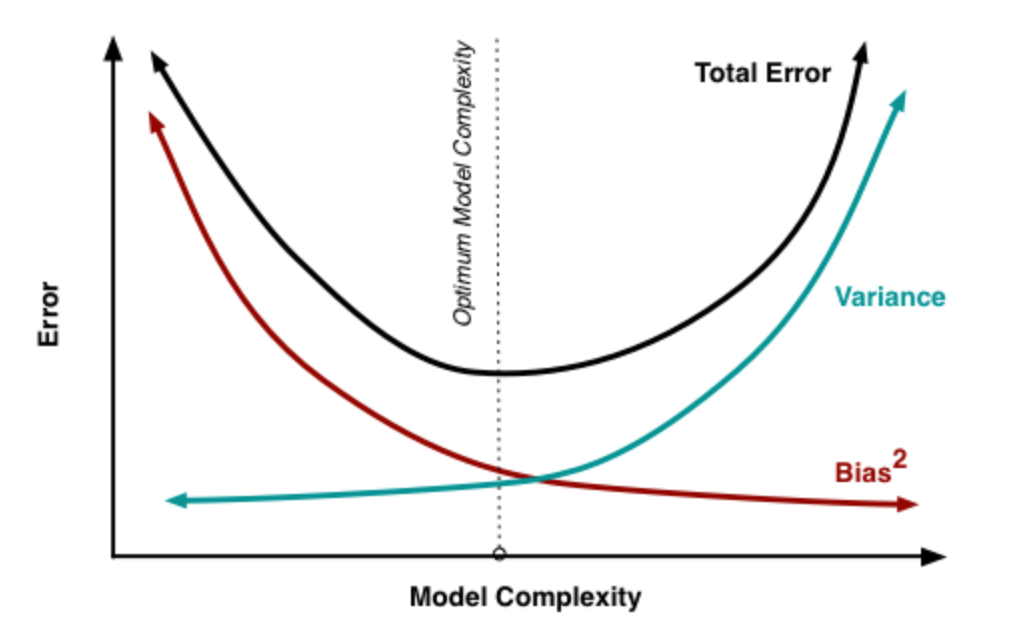
\includegraphics[width=0.4\textwidth]{figs/bias_variance1}
\caption{The bias–variance trade-off: as model complexity increases, bias decreases but variance increases.}\label{fig:bias-variance-tradeoff}
\end{figure}

\begin{figure}[H]
\begin{center}
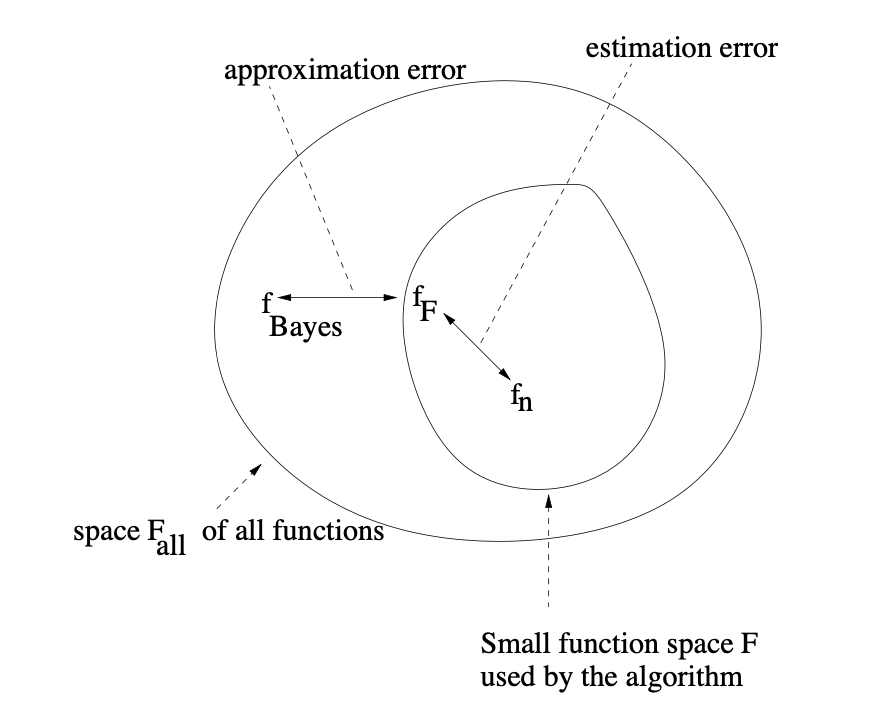
\includegraphics[width=0.5\linewidth]{figs/image2.png}
\caption{Illustration of estimation and approximation error.}\label{f2}
\end{center}
\end{figure}

\begin{figure}[H]
\begin{center}
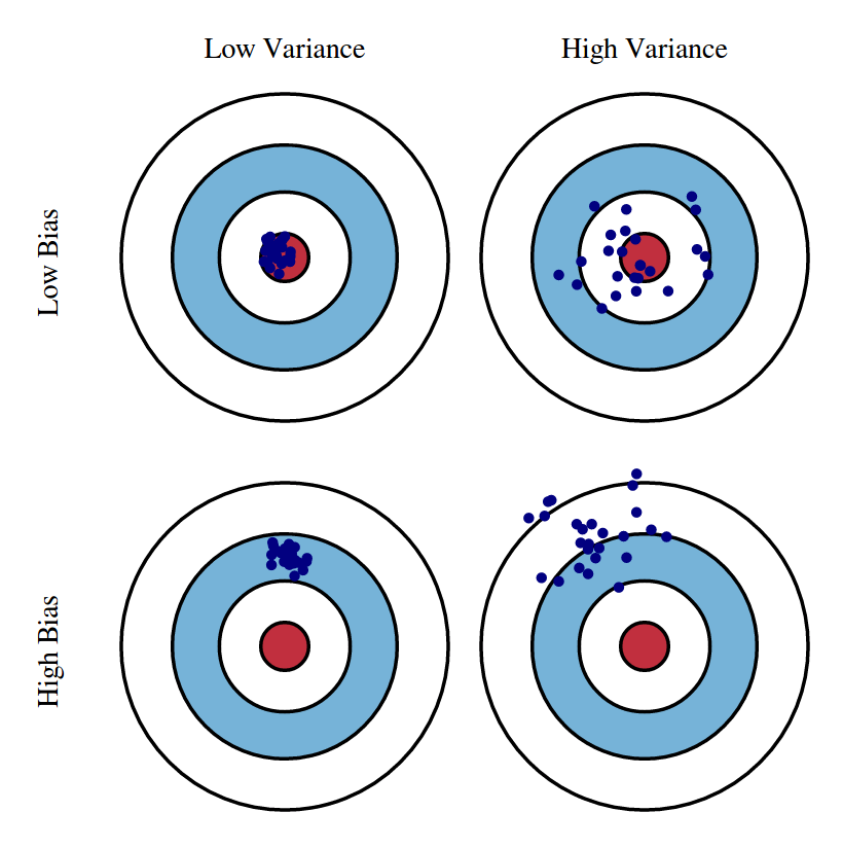
\includegraphics[width=.25\textwidth]{figs/bias_variance.png}
\caption{Graphical representation of bias and variance.}\label{f2}
\end{center}
\end{figure}

\begin{itemize}
    \item In practice, one considers nested families of hypothesis classes $\mathcal{H}_1 \subset \mathcal{H}_2 \subset \cdots$ with increasing complexity.
    \item The identification of the appropriate class (type of predictor and hyper-parameters) is called \alert{model selection}.
\end{itemize}

\subsection*{The Vapnik-Chervonenkis Dimension}

\subsubsection*{Motivation}
\begin{itemize}
    \item Finite hypothesis classes are PAC-learnable, but there exist infinite classes that are also PAC-learnable (e.g., threshold functions on $\Real$).
    \item Need a measure of complexity that captures not raw size, but how richly a class can express different labelings of data points.
    \item The \emph{Vapnik-Chervonenkis dimension} (VC-dimension) provides such a combinatorial characterization.
\end{itemize}

\subsubsection*{Restriction and Shattering}
\begin{itemize}
    \item Given a finite subset $C = \lbrace c_{1},\ldots,c_{m} \rbrace\subset \cX$, the \emph{restriction} $\cH_{C}$ of $\cH$ to $C$ is:
    \begin{myequation}
    \cH_{C} = \lbrace (h(c_{1}),\ldots,h(c_{m})): h\in\cH\rbrace
    \end{myequation}
    \item If $\cH_{C}$ contains \emph{all} $2^{|C|}$ possible binary labelings of $C$ (i.e., $|\cH_C| = 2^{|C|}$), we say $\cH$ \emph{shatters} $C$.
    \item Shattering means the class is maximally expressive on $C$: it can represent every conceivable binary classification task on those points.
\end{itemize}

\subsubsection*{VC Dimension Definition}
\begin{myequation}
\vcd{\cH} = \max\lbrace |C| : C \subset \cX,\ \cH \text{ shatters } C \rbrace
\end{myequation}
If $\cH$ shatters sets of arbitrarily large size, $\vcd{\cH} = \infty$.

\begin{itemize}
    \item The VC-dimension captures how freely a hypothesis class can label finite sets of points.
    \item If $\mathrm{VCdim}(\mathcal{H}) = d$:
    \begin{itemize}
        \item \textbf{(Existence)} There exists a set $S$ of $d$ points shattered by $\mathcal{H}$.
        \item \textbf{(Maximality)} No set of $d+1$ points can be shattered.
    \end{itemize}
    \item This is a \emph{worst-case} measure of capacity: it asks how expressive $\mathcal{H}$ can be over the most favorable configuration of points.
    \item Controlling VC-dimension is necessary for any guarantee that training performance implies test performance.
\end{itemize}

\subsubsection*{Examples}

\textbf{Threshold functions on $\Real$:} $\cH^{\text{thr}} = \{h_{\theta}(x)=\mathds{1}[x\geq\theta]\}$.
\begin{itemize}
    \item $\vcd{\cH^{\text{thr}}} \geq 1$: singleton $\{c_1\}$ can be shattered (set $\theta=c_1$ for label 1, $\theta=c_1+1$ for label 0).
    \item No set of size 2 can be shattered: for $c_1 < c_2$, labeling $(1,0)$ is impossible.
    \item Therefore $\vcd{\cH^{\text{thr}}} = 1$.
\end{itemize}

\textbf{Axis-aligned rectangles in $\Real^2$:} $\cH^{\text{rect}}$ where points inside rectangle are positive.
\begin{itemize}
    \item $\vcd{\cH^{\text{rect}}} \geq 4$: four points at cardinal extremes can be shattered.
    \item No set of size 5 can be shattered: consider bounding box and interior point.
    \item Therefore $\vcd{\cH^{\text{rect}}} = 4$.
\end{itemize}

\textbf{Interval classifiers on $\Real$:} $\cH^{\text{int}} = \{h_{a,b}(x)=\mathds{1}[a<x<b]\}$.
\begin{itemize}
    \item $\vcd{\cH^{\text{int}}} \geq 2$: $\{1,2\}$ can be shattered.
    \item No set of size 3 can be shattered: for $c_1 \leq c_2 \leq c_3$, labeling $(1,0,1)$ is impossible.
    \item Therefore $\vcd{\cH^{\text{int}}} = 2$.
\end{itemize}

\textbf{Finite hypothesis classes:}
\begin{itemize}
    \item For any finite class $\cH^{\text{fin}}$, $\vcd{\cH^{\text{fin}}} \leq \log_2 |\cH^{\text{fin}}|$.
    \item This bound can be very loose (e.g., threshold functions on $\{1,\ldots,k\}$ have $|\cH|=k$ but $\vcd{\cH}=1$).
    \item VC-dimension is a more refined and informative measure than raw size.
\end{itemize}

\subsection*{The Fundamental Theorem of Statistical Learning}

\begin{theorem}[Fundamental Theorem of Statistical Learning]
\label{thm:ftsl}
Let $\cH$ be a class of hypotheses $h:\cX\to \{0,1\}$ for binary classification with $0$-$1$ loss. Let $d = \vcd{\cH}$. Then the following statements are equivalent:
\begin{enumerate}
    \item $\cH$ has a finite VC-dimension: $d < \infty$.
    \item $\cH$ is \textbf{agnostic PAC-learnable}, and there exist absolute constants $c_1 < c_2$ such that:
    \begin{myequation}
    \frac{c_1}{\varepsilon^2}\!\left(d+\ln\frac{1}{\delta}\right)
    \;\leq\;
    m_\cH(\varepsilon, \delta)
    \;\leq\;
    \frac{c_2}{\varepsilon^2}\!\left(d+\ln\frac{1}{\delta}\right)
    \end{myequation}
    Moreover, ERM is a successful agnostic PAC-learning algorithm for $\cH$.
    \item $\cH$ is \textbf{PAC-learnable} (under realizability), and there exist absolute constants $c_1 < c_2$ such that:
    \begin{myequation}
    \frac{c_1}{\varepsilon}\!\left(d+\ln\frac{1}{\delta}\right)
    \;\leq\;
    m_\cH(\varepsilon, \delta)
    \;\leq\;
    \frac{c_2}{\varepsilon}\!\left(d+\ln\frac{1}{\delta}\right)
    \end{myequation}
    Moreover, ERM is a successful PAC-learning algorithm for $\cH$.
\end{enumerate}
\end{theorem}

\begin{itemize}
    \item \textbf{The role of $d$:} Sample complexity grows linearly in VC-dimension $d$ and logarithmically in $1/\delta$.
    \item \textbf{Matching upper and lower bounds:} Sample complexity is tight up to absolute constants $c_1$ and $c_2$.
    \item \textbf{The $1/\varepsilon^2$ vs $1/\varepsilon$ gap:} Reflects fundamental statistical difficulty — in the agnostic setting, distinguishing the best hypothesis from near-competitors requires substantially more data.
    \item \textbf{ERM as a universal learner:} ERM works universally across all classes with finite VC-dimension (statistical guarantee; computational cost may still be intractable).
    \item \textbf{Infinite VC dimension:} Follows from NFL theorem — $\mathrm{VCdim}(\mathcal{H}) = \infty$ implies unlearnability.
\end{itemize}

\subsection*{From the Fundamental Theorem to the VC Generalization Bound}

\begin{itemize}
    \item The VC generalization bound makes precise how VC-dimension controls the gap between training and true performance.
    \item With probability at least $1-\delta$ over the random draw of the training sample, \emph{every} $h \in \cH$ simultaneously satisfies:
    \begin{equation}
    \label{eq:vcbound}
    L_{\mathcal{D}}(h) \;\le\; \hat{L}(h) \;+\;
    O\!\left(\sqrt{\frac{d\log(n/d) + \log(1/\delta)}{n}}\right)
    \end{equation}
    where $\hat{L}(h)$ is empirical error and $L_{\mathcal{D}}(h)$ is true error.
\end{itemize}

\subsubsection*{Structure of the Bound}
\[
\underbrace{L_{\mathcal{D}}(h)}_{\text{generalization error}}
\;\le\;
\underbrace{\hat{L}(h)}_{\text{training error}}
\;+\;
\underbrace{\Phi(d,n,\delta)}_{\text{complexity term}}
\]

\begin{itemize}
    \item The complexity term $\Phi$ decreases as $O(1/\sqrt{n})$ with more data and grows with VC-dimension $d$.
    \item The bound holds \emph{uniformly} over all $h \in \cH$, making it applicable to the output of ERM.
\end{itemize}

\subsubsection*{Derivation Sketch}
\begin{enumerate}
    \item \textbf{Challenge of uniform convergence:} For a fixed hypothesis, Hoeffding gives $P(|L_\mathcal{D}(h) - \hat{L}(h)| > \varepsilon) \leq 2e^{-2n\varepsilon^2}$. Need this for all $h \in \cH$ simultaneously.
    \item \textbf{Symmetrization:} Introduce ghost sample $S'$ to reduce problem to controlling $\cH$ on finite set $S \cup S'$ of $2n$ points.
    \item \textbf{Growth function and Sauer-Shelah lemma:} Define $\Pi_\cH(m) = \max_{|S|=m} |\{(h(x_1),\ldots,h(x_m)) : h \in \cH\}|$. If $\vcd{\cH} = d$, Sauer-Shelah lemma gives $\Pi_\cH(m) \leq \sum_{i=0}^{d} \binom{m}{i} \leq \left(\frac{em}{d}\right)^d$.
    \item \textbf{Combining bounds:} Union bound over $\Pi_\cH(2n)$ distinct labelings yields:
    \begin{myequation}
    \Pr_S\!\left[\sup_{h \in \cH} \bigl(L_\mathcal{D}(h) - \hat{L}_S(h)\bigr) > \varepsilon\right]
    \;\le\;
    4\left(\frac{2en}{d}\right)^d e^{-n\varepsilon^2/8}
    \end{myequation}
    \item Setting this probability equal to $\delta$ and solving for $\varepsilon$ gives the bound~\eqref{eq:vcbound}.
\end{enumerate}

\begin{itemize}
    \item The $d\log(n/d)$ term arises from the logarithm of the Sauer-Shelah bound, representing the search cost over effective hypotheses.
    \item The $\log(1/\delta)$ term ensures the desired confidence level.
    \item Finite VC-dimension forces $\cH$ to be effectively finite on any finite sample, making uniform convergence possible.
    \item When $d = \infty$, the growth function may grow as $2^n$, uniform convergence fails, and learning is impossible.
\end{itemize}

\subsection*{Summary}
\begin{itemize}
    \item Statistical learning theory provides a complete characterization of when binary classification is learnable.
    \item The VC-dimension is the exact combinatorial quantity that determines learnability:
    \begin{itemize}
        \item Finite VC-dimension $\iff$ PAC learnability (both realizable and agnostic).
        \item Sample complexity scales as $O(d/\varepsilon^2)$ in the agnostic case and $O(d/\varepsilon)$ in the realizable case, with logarithmic dependence on $1/\delta$.
    \end{itemize}
    \item ERM is a universal learning algorithm for any class with finite VC-dimension.
    \item The VC generalization bound provides the quantitative relationship between training error, VC-dimension, sample size, and generalization error.
    \item The No-Free-Lunch theorem establishes that without inductive bias (restricting the hypothesis class), learning is impossible.
    \item The bias-variance trade-off captures the fundamental tension in model selection: choosing a hypothesis class that balances approximation error and estimation error.
\end{itemize}
